\documentclass{article}

\usepackage{graphicx}
\usepackage{pgfplots}
\usepackage{subcaption}

\title{Text symbol classification using neural networks}
\author{Kacper Ochnik \and Paweł Frankowski}
\date{\today}

\begin{document}

\begin{titlepage}
	\centering
	
\includegraphics[width=0.3\textwidth]{Logo_PK_kolor_EN_PNG.png}\par\vspace{1cm}
	{\textsc{Koszalin University of Technology} \par}
	\vspace{1cm}
	{\Large \textsc{Applications of artificial intelligence project report}\par}
	\vspace{1.5cm}
	{\huge\bfseries Handwritten text symbol recognition with deep neural networks
	\par}
	\vspace{2cm}
	{\Large\itshape {Paweł Frankowski \space Kacper Ochnik}\par}
	\vfill
	supervised by\par
	Dr.~Adam Słowik

	\vfill

	{\large \today\par}
\end{titlepage}

\tableofcontents
\newpage

\section{Introduction - Kacper}
Handwritten text symbol recognition with deep neural networks.

\newpage
\section{Our goal - Pawel  [Done]}

The primary objective of our project is to develop a handwritten text symbol recognition system using deep neural networks. We aimed to create a model capable of accurately identifying and classifying handwritten digits ranging from 0 to 9 on a matrix of 28x28 pixels.

\subsection{Specific objectives}

In pursuit of our overarching goal, we have identified the following specific objectives:

\begin{enumerate}
    \item \textbf{Project setup} - Set up the project environment and install the necessary libraries and packages.
    \item \textbf{Code implementation} - Write Python code to implement the deep neural network architecture. This includes developing modules for data preprocessing, model training, and evaluation.
    \item \textbf{Data Collection} - Gather a comprehensive dataset of handwritten digits (0 to 9) in a 28x28 pixel matrix format from MNIST.
	\item \textbf{Learning} - Train the model using the collected dataset.
	\item \textbf{Optimization} - Improve the model's accuracy through optimization techniques. Accelerate computational efficiency for faster calculations.
    \item \textbf{Testing} - Create testing GUI for the trained model. Evaluate the model's performance metrics.
	\item \textbf{Documentation} - Write a comprehensive report documenting the project's objectives, methodology, and outcomes.
\end{enumerate}

\subsection{Expected Outcomes}

Upon successful completion of our project, we anticipate achieving the following outcomes:

\begin{itemize}
    \item Develop a robust deep neural network model capable of recognizing and classifying handwritten digits from 0 to 9.
    \item Train the model to achieve a acceptable level of accuracy.
\end{itemize}

\newpage
\section{Decision boundary - Kacper}
...

\newpage
\section{Weights and Biases - Pawel  [Done]}
Weights are indicators of the importance of the input in predicting the final output. Biases are essential as they allow the network to have some flexibility in fitting the data. In the training process of our neural network, the weights and biases play a crucial role in determining the model's performance. Here, we discuss the initialization, calculation, and adjustment of weights and biases in the network. 

\subsection{Initialization}
The \texttt{Layer} class represents a single layer in the neural network. It contains information about the number of nodes in and out, weights, biases, and gradients. The neural network is initialized with random weights using the Xavier/Glorot initialization technique. This method helps in achieving better convergence during training.

\begin{figure}[h]
    \centering 
    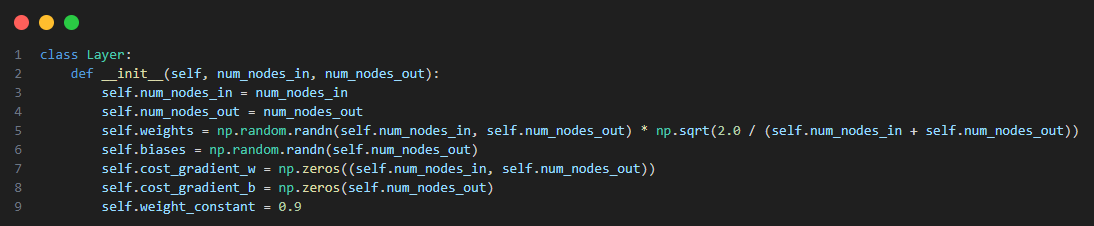
\includegraphics[width=1\textwidth]{images/Xavier-Glorot-initialization-for-weights.png}
    \caption{Initialization of random biases and weights using Xavier/Glorot technique}
    \label{fig:initialized_weights}
\end{figure}

When a neural network is first trained, it is first fed with input. Since it isn't trained yet, we don't know which weights should we use for each input. And so, each input is randomly assigned a weight. It will very likely give incorrect output.

\subsection{Weighted sum of inputs}
In the \texttt{Layer} class, the calculation of outputs begins with the computation of weighted inputs. For each node in the layer, the weighted inputs are calculated using the formula.:
\begin{figure}[h]
    \centering
    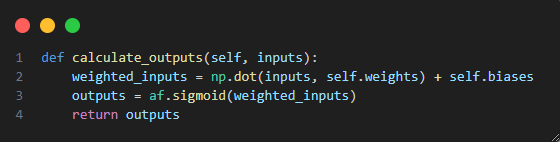
\includegraphics[width=1\textwidth]{images/dot-product-of-inputs-and-weights.png}
    \caption{The dot product of inputs and weights, representing the weighted sum of inputs}
    \label{fig:weighted_sum}
	\subcaption*{The \texttt{calculate outputs} method calculates the dot product of inputs and weights, representing the weighted sum of inputs. The biases are then added to this sum to introduce flexibility in fitting the data. Finally, the result is passed through the sigmoid activation function to introduce non-linearity to the model, and the outputs are obtained.}
\end{figure}

\newpage
\section{Hidden layers - Kacper}
...

\newpage
\section{Activation functions - Pawel [Done]}
Activation functions play a crucial role in neural networks, introducing non-linearity to the model and allowing it to learn complex relationships in the data. Here, we describe various activation functions implemented in the \texttt{activation functions} module.

\subsection{Sigmoid function}
The sigmoid function squashes its input to the range (0, 1), making it suitable for binary classification problems.

\begin{equation}
	f(x) = \frac{1}{1 + e^{-x}}
\end{equation}

\begin{equation}
    \begin{tikzpicture}
        \begin{axis}[
            xlabel={$x$},
            ylabel={$f(x)$},
            domain=-5:5,
            samples=100,
            smooth,
            scale=1.5
        ]
            \addplot[blue] {1/(1 + exp(-x))};
            \legend{$f(x) = \frac{1}{1 + e^{-x}}$}
        \end{axis}
    \end{tikzpicture}
\end{equation}

\begin{figure}[h]
    \centering
    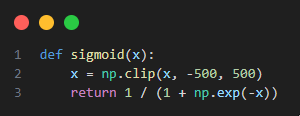
\includegraphics[width=0.5\textwidth]{images/sigmoid-function.png}
    \caption{Sigmoid function}
    \label{fig:sigmoid_function}
	\subcaption*{Limiting the values of x to prevent overflow. Overflow refers to a situation where the exponential function in the sigmoid formula produces very large positive values, causing numerical instability in calculations. The exponential function, especially when dealing with large positive inputs, can lead to floating-point overflow, which means the result becomes too large to be represented within the numerical precision of the system.}
\end{figure}

\subsection{The derivative of the sigmoid function}
The derivative of the sigmoid function is used in the backpropagation algorithm to calculate the gradients of the cost function with respect to the weights and biases. The derivative of the sigmoid function is given by the formula:

\begin{equation}
    f'(x) = f(x) \cdot (1 - f(x))
\end{equation}

\begin{figure}[h]
    \centering
    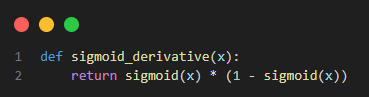
\includegraphics[width=0.5\textwidth]{images/sigmoid-derivative.png}
    \caption{The derivative of the sigmoid function}
    \label{fig:sigmoid_derivativse_function}
\end{figure}

\newpage
\section{Cost function - Kacper}
...

\newpage
\section{Gradient descent - Pawel}
The cost gradients for weights and biases are initialized with zeros, and during training, these gradients will be updated based on the backpropagation algorithm.

\begin{figure}[h]
    \centering 
    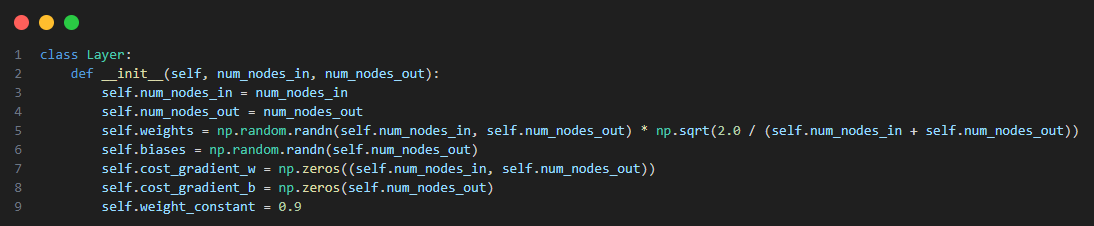
\includegraphics[width=1\textwidth]{images/Xavier-Glorot-initialization-for-weights.png}
    \caption{Initialization a vector of zeros with the same length as the bias vector}
    \label{fig:initialized_cost_gradient}
	\subcaption*{This matrix will be used to accumulate the gradients of the cost function with respect to the weights during the backpropagation process.	}
\end{figure}

\newpage
\section{Cost landscape - Kacper}
...

\newpage
\section{Learning algorithm - naive approach - Pawel}
...

\newpage
\section{Learning algorithm - calculus approach - Kacper}
...

\newpage
\section{Learning algorithm - digit recognition - Pawel}
...

\newpage
\section{Chain rule - Pawel/Kacper}
...

\newpage
\section{Backpropagation - Kacper}
...

\newpage
\section{Testing the network - Kacper}
...

\newpage
\section{Conclusion - Pawel}
This is the conclusion of the document.

\end{document}
